

%
% Figure 1-- Dectector End View plus event
%
\begin{figure}[!ht]
\centering
%\includegraphics[angle=0,width=0.65\textwidth]{Figures/Detector_end_view.jpg}
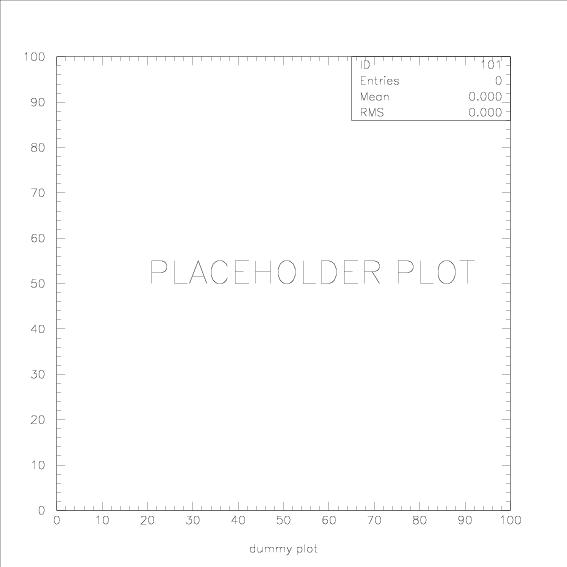
\includegraphics[angle=0,width=0.65\textwidth]{Figures/dummy.jpg}
\caption{A sketch of a low-Z whole-body PET scanner with a simulated annihilation event from TOPAS superimposed. The location of the annihilation is indicated by the star; the successive interactions in the detector by Compton scattering are indicated by the resulting electron tracks in the low-Z medium. The location of the first scatter of each gamma determines the corresponding end of the Line-of-Response, with the goal of a transverse resolution measured in tens of microns~\cite{PET_NIM_paper}. The superposition of many lines of response gives a point-spread function with the transverse resolution~\cite{PET_NIM_paper}
.}
\label{fig:Detector_end_view}
\end{figure}


%\vspace*{-1.5in}
% Figure 2: the Compton Chain
%
\begin{figure}[!ht]
\centering
%\includegraphics[angle=0,width=0.65\textwidth]{Figures/Compton_chain.jpg}
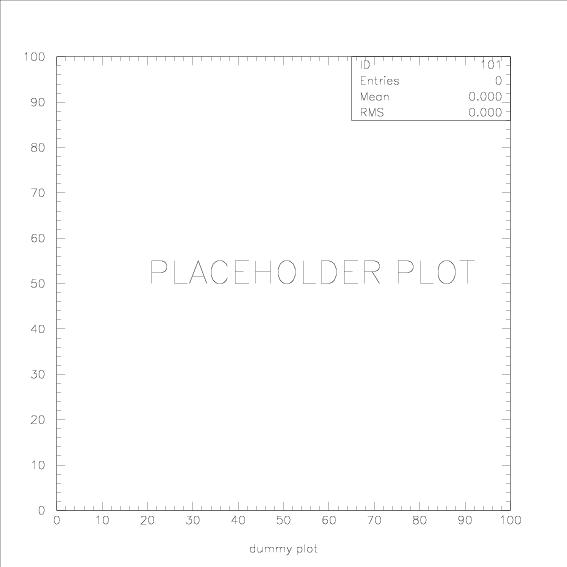
\includegraphics[angle=0,width=0.65\textwidth]{Figures/dummy.jpg}
\caption{The location, time, deposited energy, and track of the scattered electron of successive Compton scatterings in a detector module as simulated with the TOPAS tools. The scattering angles of the gamma and the energy of the scattered electron are determined by conservation of energy and momentum in the 2-body Compton process, providing handles on reconstructing the correct time-ordering. The earlier (higher energy) end of an electron track can be statistically determined from energy deposition and angular scattering. There are additional constraints from the requirement that the LOR connecting the 2 first-scatters must lie in the plane of the scattering determined by the angles and the electron track, and the angle between the two planes has a dependence predicted by the quantum entanglement of the two gamma polarizations. The TOF system may provide additional information constraining the time-ordering of the creation of the electrons. }
\label{fig:Compton_Chain}
\end{figure}
